\documentclass[border=0pt]{standalone}
\usepackage{tikz}
\usetikzlibrary{arrows.meta}
\begin{document}
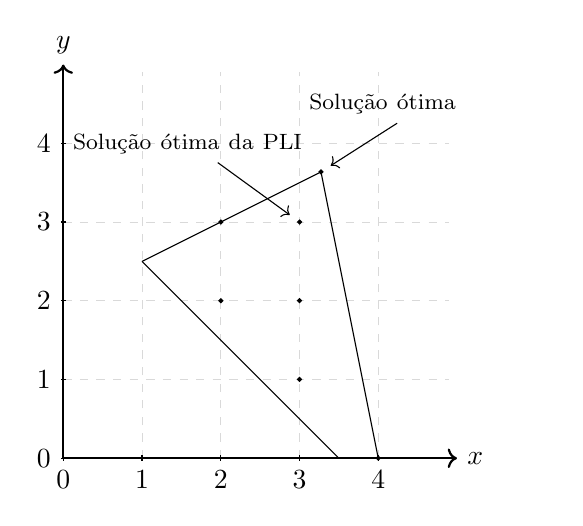
\begin{tikzpicture}

    \draw[help lines, color=gray!30, dashed] (0, 0) grid (4.9,4.9);
    \draw[->,thick] (0,0)--(5,0) node[right]{$x$};
    \draw[->,thick] (0,0)--(0,5) node[above]{$y$};

    \draw (1.0   , 2.5   ) -- (3.2727, 3.6363); % Linha de cima
    \draw (3.2727, 3.6363) -- (4.0   , 0     ); % Linha da direita
    \draw (4.0   , 0.0   ) -- (3.5   , 0     ); % Linha de baixo
    \draw (3.5   , 0.0   ) -- (1.0   , 2.5   ); % Linha da esquerda

    \draw [fill] (2, 3) circle [radius=.025];
    \draw [fill] (2, 2) circle [radius=.025];

    \draw [fill] (3, 3) circle [radius=.025];
    \draw [fill] (3, 2) circle [radius=.025];
    \draw [fill] (3, 1) circle [radius=.025];

    \draw [fill] (4, 0) circle [radius=.025];

    \draw [fill] (3.2727, 3.6363) circle [radius=.025];

    \node (1) at (3.2727, 3.6363) {};
    \node (2) [text width=3cm, above, right] at (3, 4.5) {\footnotesize Solu\c{c}\~ao \'otima};

    \node (3) at (3, 3) {};
    \node (4) [text width=3cm, above, right] at (0, 4.0) {\footnotesize Solu\c{c}\~ao \'otima da PLI};

    \path [->] (2) edge node {} (1);
    \path [->] (4) edge node {} (3);

    \foreach \x in {0,1,2,3,4}
        \draw (\x cm,1pt) -- (\x cm,-1pt) node[anchor=north] {$\x$};
    \foreach \y in {0,1,2,3,4}
        \draw (1pt,\y cm) -- (-1pt,\y cm) node[anchor=east] {$\y$};

\end{tikzpicture}
\end{document}
